\section{Configuration Spaces}
\begin{quote}
Just as one can compose colors or forms, so one can compose motions.
\end{quote}
{\raggedright{}Alexander Calder, 1933}


We described the configuration space of a linkage earlier and have introduced polygonal linkages and disk arrangements without describing their corresponding definitions of a configuration space.  Here we will describe configuration spaces for each structure.

% We'd like to describe motions and range of motions of embedded graphs, linkages, polygonal 
% linkages, and disk arrangements.  Table \ref{table:configurationSpace-1} provides the definition of 
% \textit{reconfiguration} for each type of object covered so far:
% \begin{center}
% \begin{table}[htbp!]
% \begin{tabular}{|p{.2\textwidth}|p{.79\textwidth}|}
% \hline
% Object Type&Definition of Reconfiguration\\\hline
% Graph Embeddings&a continuous motion of the vertices that never causes the edges to 
% intersect.\\\hline
% Linkage&a continuous motion of the vertices that preserves the lengths of the edges and never 
% causes 
% the edges to intersect.\\\hline
% Polygonal Linkage&a continuous motion of polygons that preserves shapes of polygons, hinge point 
% pairings, and never causes the polygonal sides to intersect.\\\hline
% Disk Arrangement&a continuous motion of disks that preserves disk radii, pairs of contact points, 
% and never causes disks to intersect.\\\hline
% \end{tabular}\label{table:configurationSpace-1}
% \end{table}
% \end{center}




% For graphs, a \textit{reconfiguration} is a continuous motion of 
% the vertices that preserve the length edges and never cause edges to collide \cite{AKR+04}.  For 
% polygonal linkages, a reconfiguration is 


 
 \subsection{Configuration Spaces of Polygonal Linkages}
Recall a realization of a polygonal linkage is an interior-disjoint placement of 
congruent copies of the polygons in $\PP$ such that the copies of a hinge are mapped to the same point (e.g., Figure \ref{fig:linkage-1}).
First consider the set of all realizations for the polygonal linkage. $\left(\PP,\HH
\right)$ and call it $P$.  For any realization $R \in P$, the parameterization $\mu:R \mapsto \bbR^{2m}$ where $m$ is the number of distinct vertices in $\PP$.     The configuration space is the set $\mu(P)$.

 \subsection{Configuration Spaces of Disk Arrangements}
%show an equivalent disk arrangment to the geometric dissection in thier corresponding/equivalent
% configurations.
Consider the set of realizations $P$ for a given disk arrangement $\DD = \left\lbrace D_i \right\rbrace_{i=1}^n$.  For any realization $R \in P$, there exists a corresponding contact graph, $C$.  The configuration spaces of $\DD$ are sets of $R \in P$ that are classified by the equivalent contact graphs, i.e. if $R_1$, $R_2 \in P$ and their corresponding contact graphs $C_1$ and $C_2$ have a graph isomorphism, $\phi$, then $R_1$ and $R_2$ belong to the same configuration space.



\begin{figure}[!h]
\begin{center}
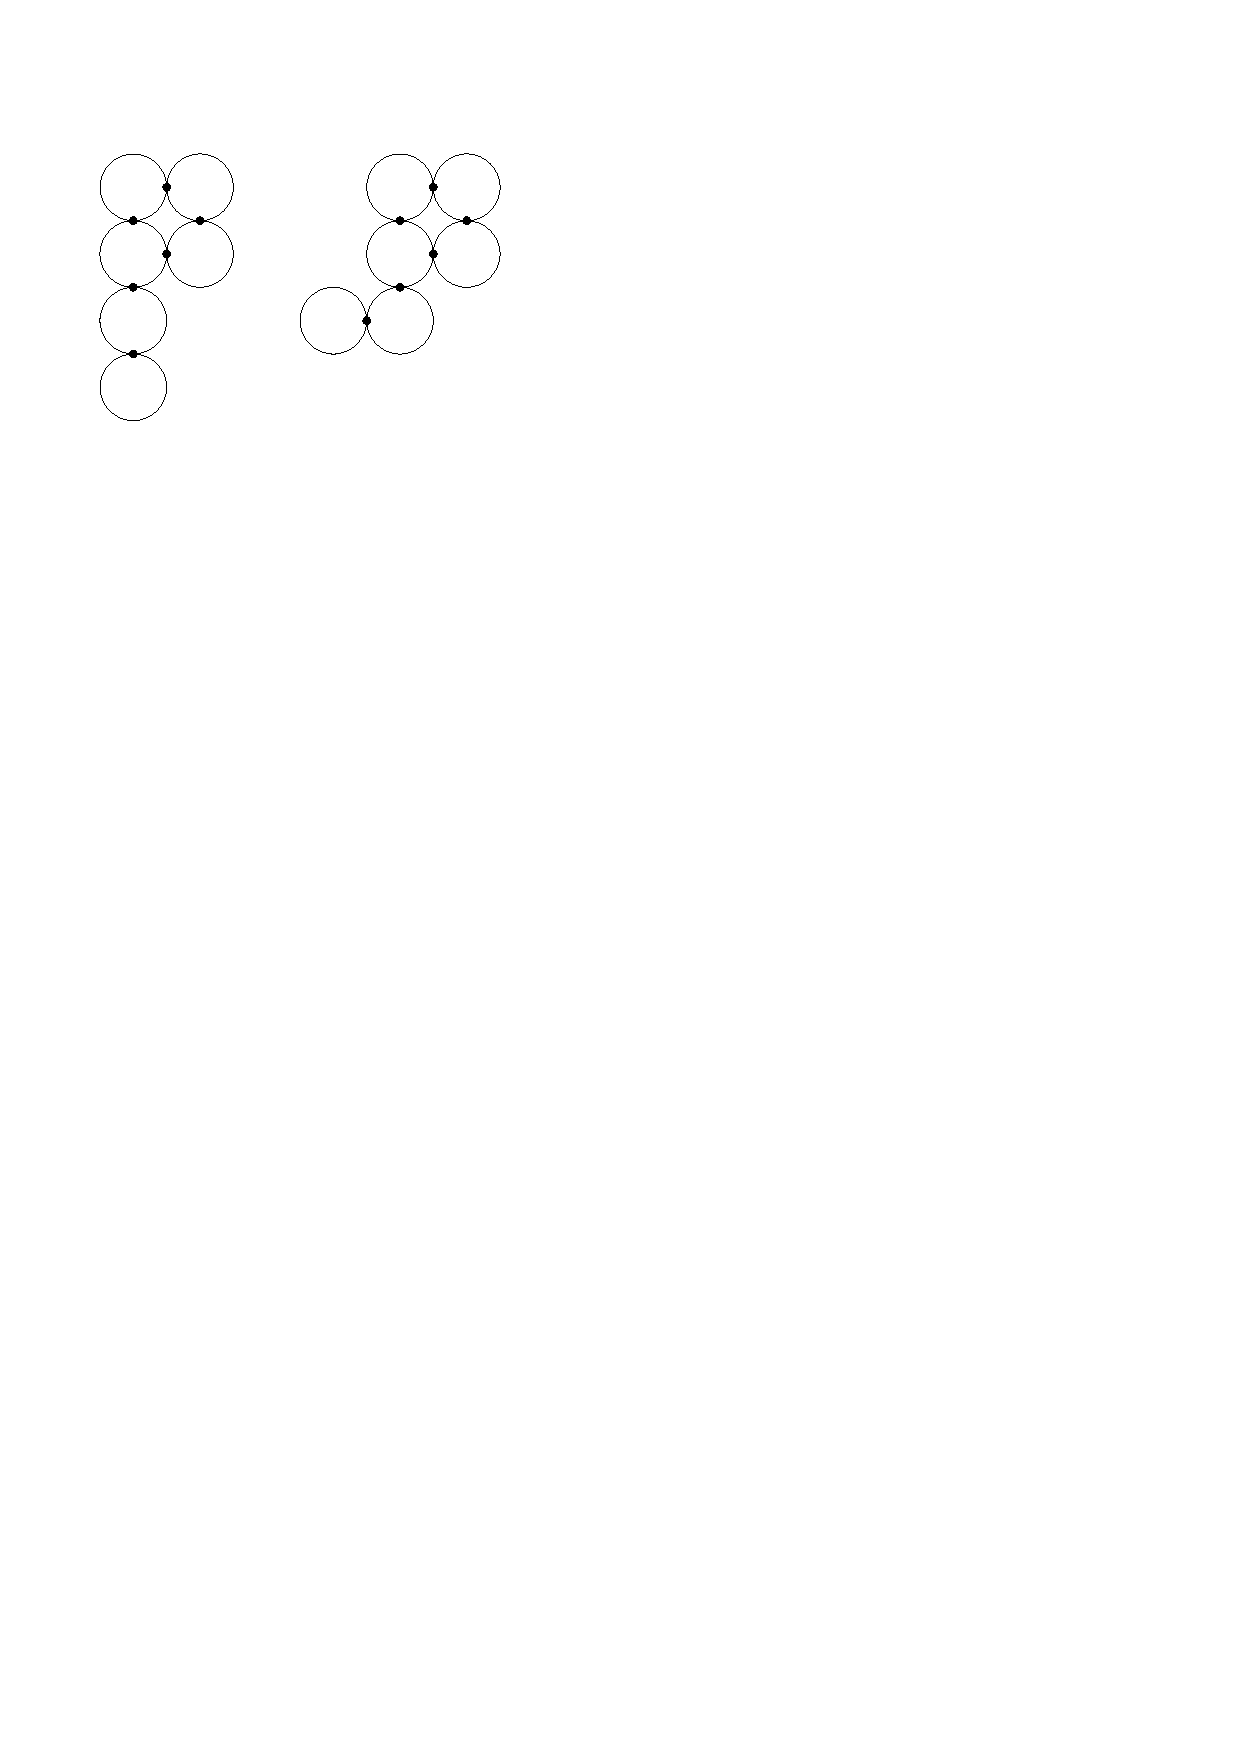
\includegraphics[scale=.75]{graphics/DiskPackingReconfiguration.pdf}
\end{center} 
\caption{A linkage whose complete configuration space is discontinuous.  These two examples above 
are two configurations of the same linkage that cannot continuously transform into the other 
without edge crossing.}
\label{fig:configuration-5}
\end{figure}

\subsection{Reconfiguration}



We'd like to describe motions and range of motions of embedded graphs, linkages, polygonal 
linkages, and disk arrangements.  Table \ref{table:configurationSpace-1} provides the definition of 
\textit{reconfiguration} for each type of object covered so far:
\begin{center}
\begin{table}[htbp!]
\begin{tabular}{|p{.2\textwidth}|p{.79\textwidth}|}
\hline
Object Type&Definition of Reconfiguration\\\hline
Graph Embeddings&a continuous motion of the realized vertices that never causes the edges to 
intersect.\\\hline
Linkage&a continuous motion of the realized vertices that preserves the lengths of the edges and never 
causes 
the edges to intersect.\\\hline
Polygonal Linkage&a continuous motion of polygons that preserves shapes of polygons, hinge point 
pairings, and never causes the polygonal sides to intersect.\\\hline
Disk Arrangement&a continuous motion of disks that preserves disk radii, pairs of contact points, 
and never causes disks to intersect.\\\hline
\end{tabular}\label{table:configurationSpace-1}
\end{table}
\end{center}








% 
% \paragraph{Confining Linkages to a Restricted Space Within a Configuration Space}
% So we've covered the idea of linkages within a plane; now let's constrain the plane to a strip and 
% have a linkage that is a \textit{polygon}, i.e. a linkage that forms a closed chain (e.g. Table 
% \ref{table:linkage-1}), hugging the boundaries of the strip:
% \begin{figure}[h]
% \begin{center}
%   ~ %add desired spacing between images, e. g. ~, \quad, \qquad etc.
%     %(or a blank line to force the subfigure onto a new line)
%   \begin{subfigure}[b]{0.49\textwidth}
% 	  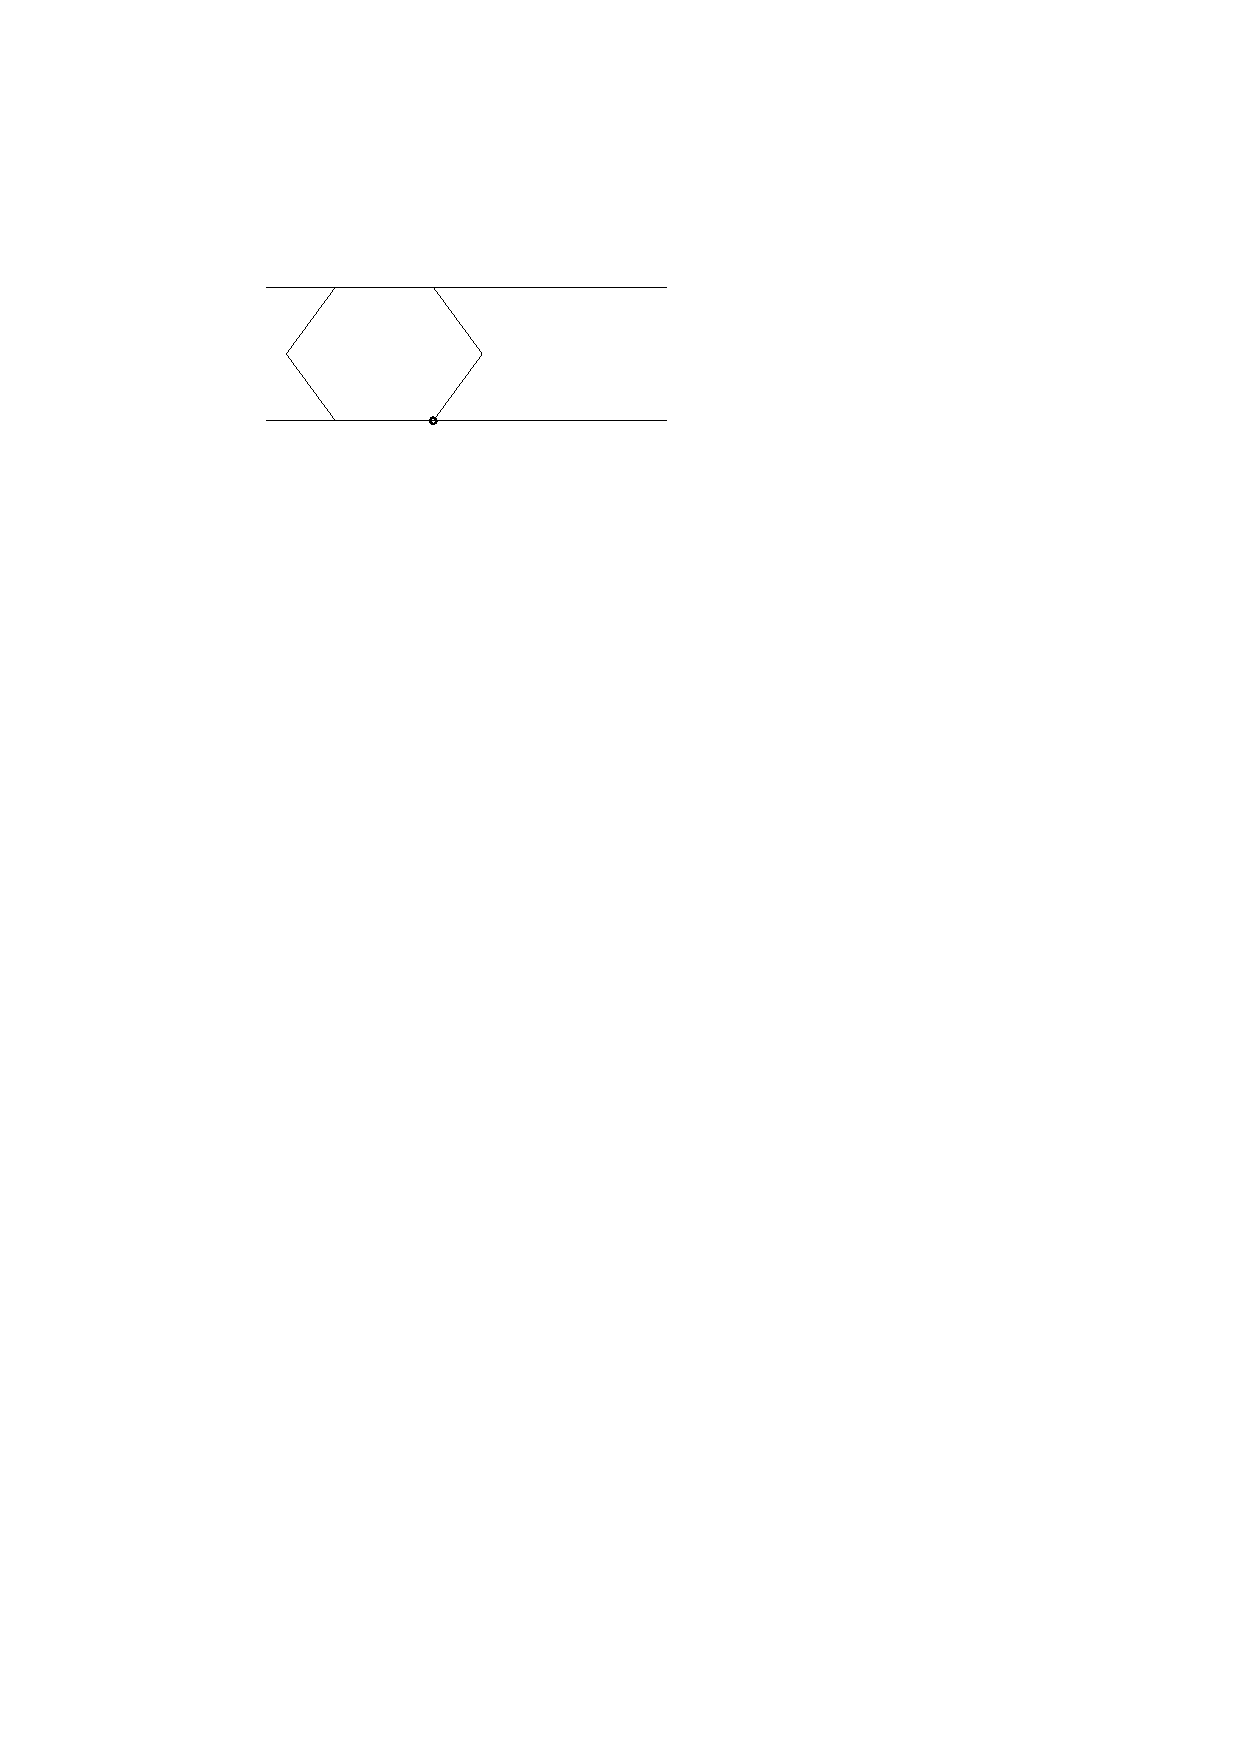
\includegraphics[width=\textwidth]{graphics/hexagonInChannelWithPinnedJointRight.pdf}
% 	  \caption{A bounded hexagon that resides in a channel with a pinned vertex}
% 	  \label{fig:linkage-1-1}
%   \end{subfigure}
%   \begin{subfigure}[b]{0.49\textwidth}
% 	  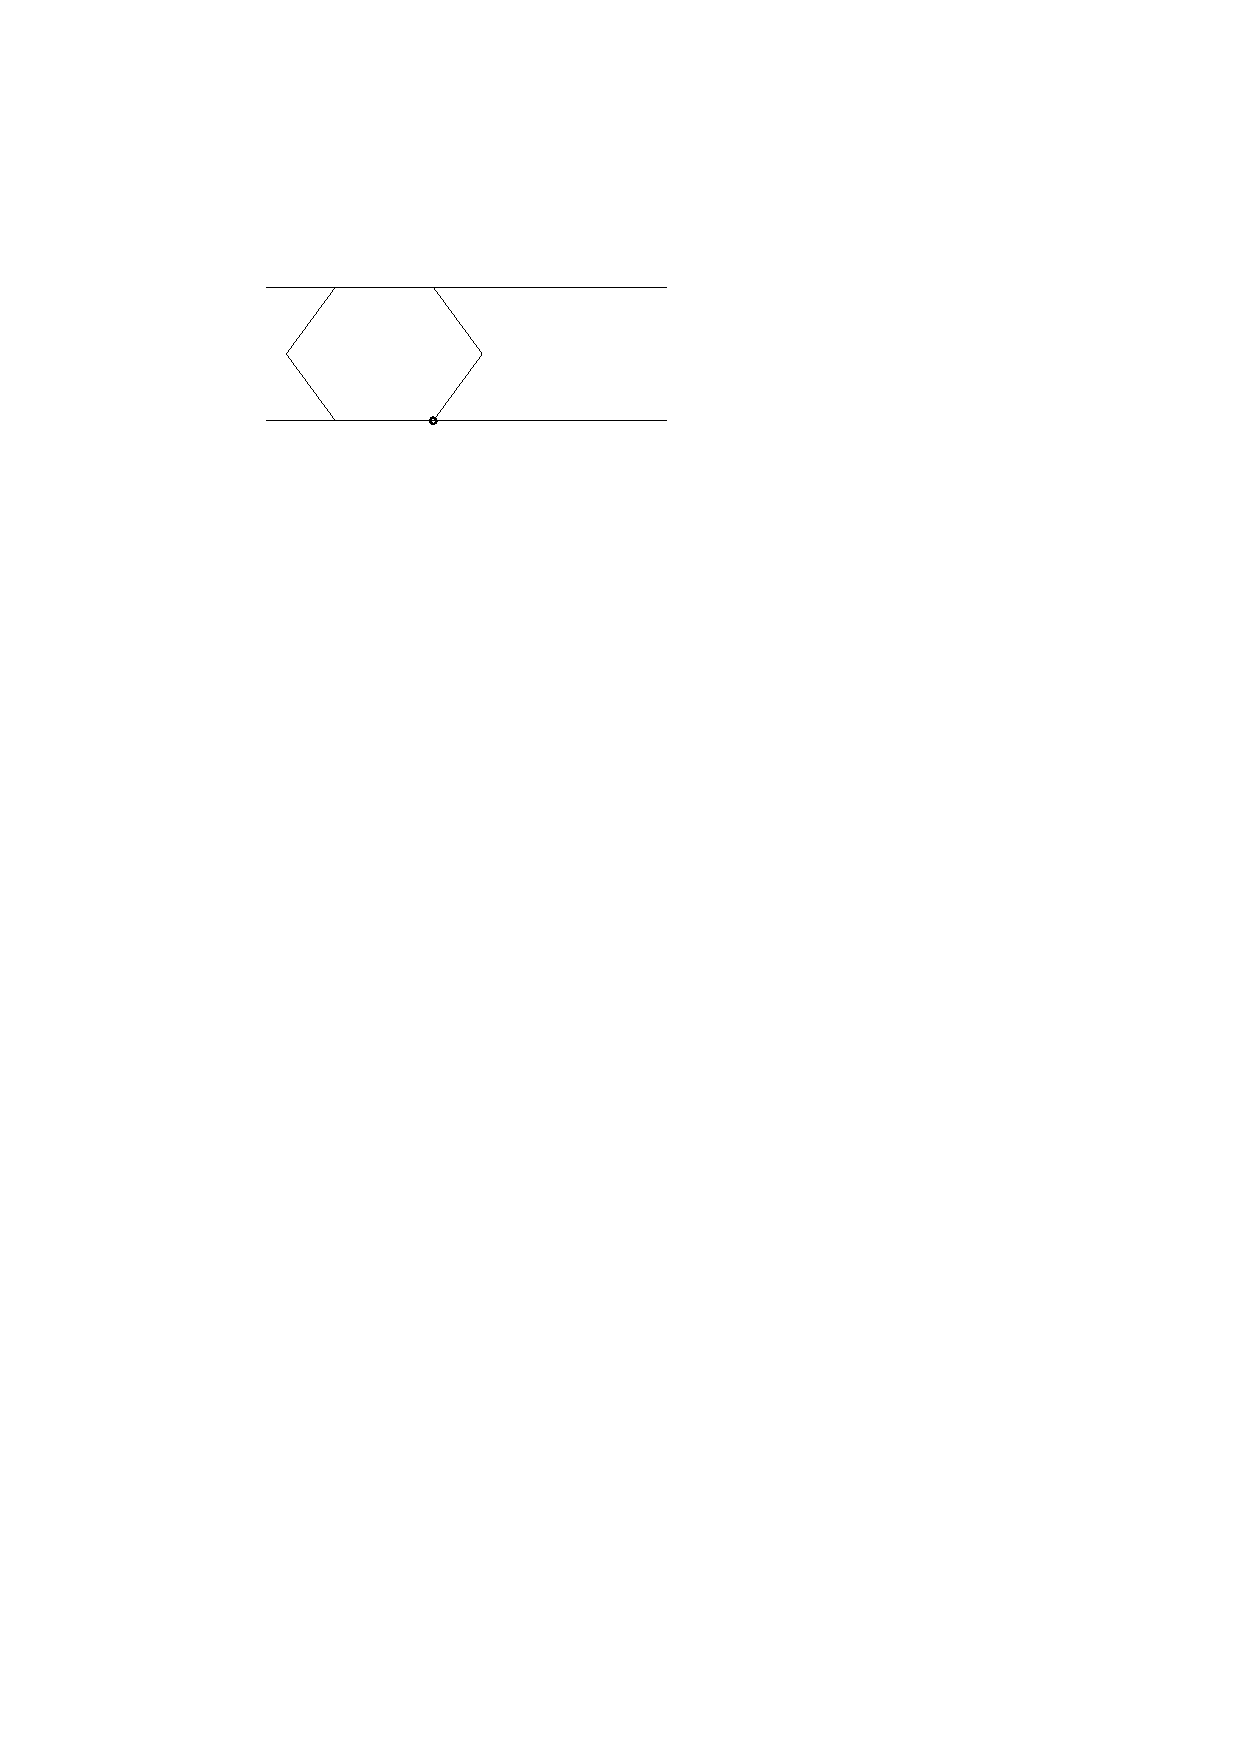
\includegraphics[width=\textwidth]{graphics/hexagonInChannelWithPinnedJointLeft.pdf}
% 	  \caption{The second realization of the hexagon residing in a channel with a pinned 
% vertex.}
% 	  \label{fig:linkage-1-2}
%   \end{subfigure}
% \end{center} 
% \caption{Due to the strip in the plane that the hexagon is bounded within the configuration space is 
% limited to just two realizations.}\label{fig:linkage-1}
% \end{figure}
% So here we have a linkage whose conifguration space is limited to just two realizations.  With just 
% two realizations, we can assign a binary value to them and have the linkage act as a boolean 
% variable.  We will revisit this concept when we cover satisfiability problems later on in the paper.
% \begin{figure}[h]
% \begin{center}
%   ~ %add desired spacing between images, e. g. ~, \quad, \qquad etc.
%     %(or a blank line to force the subfigure onto a new line)
%   \begin{subfigure}[b]{0.49\textwidth}
% 	  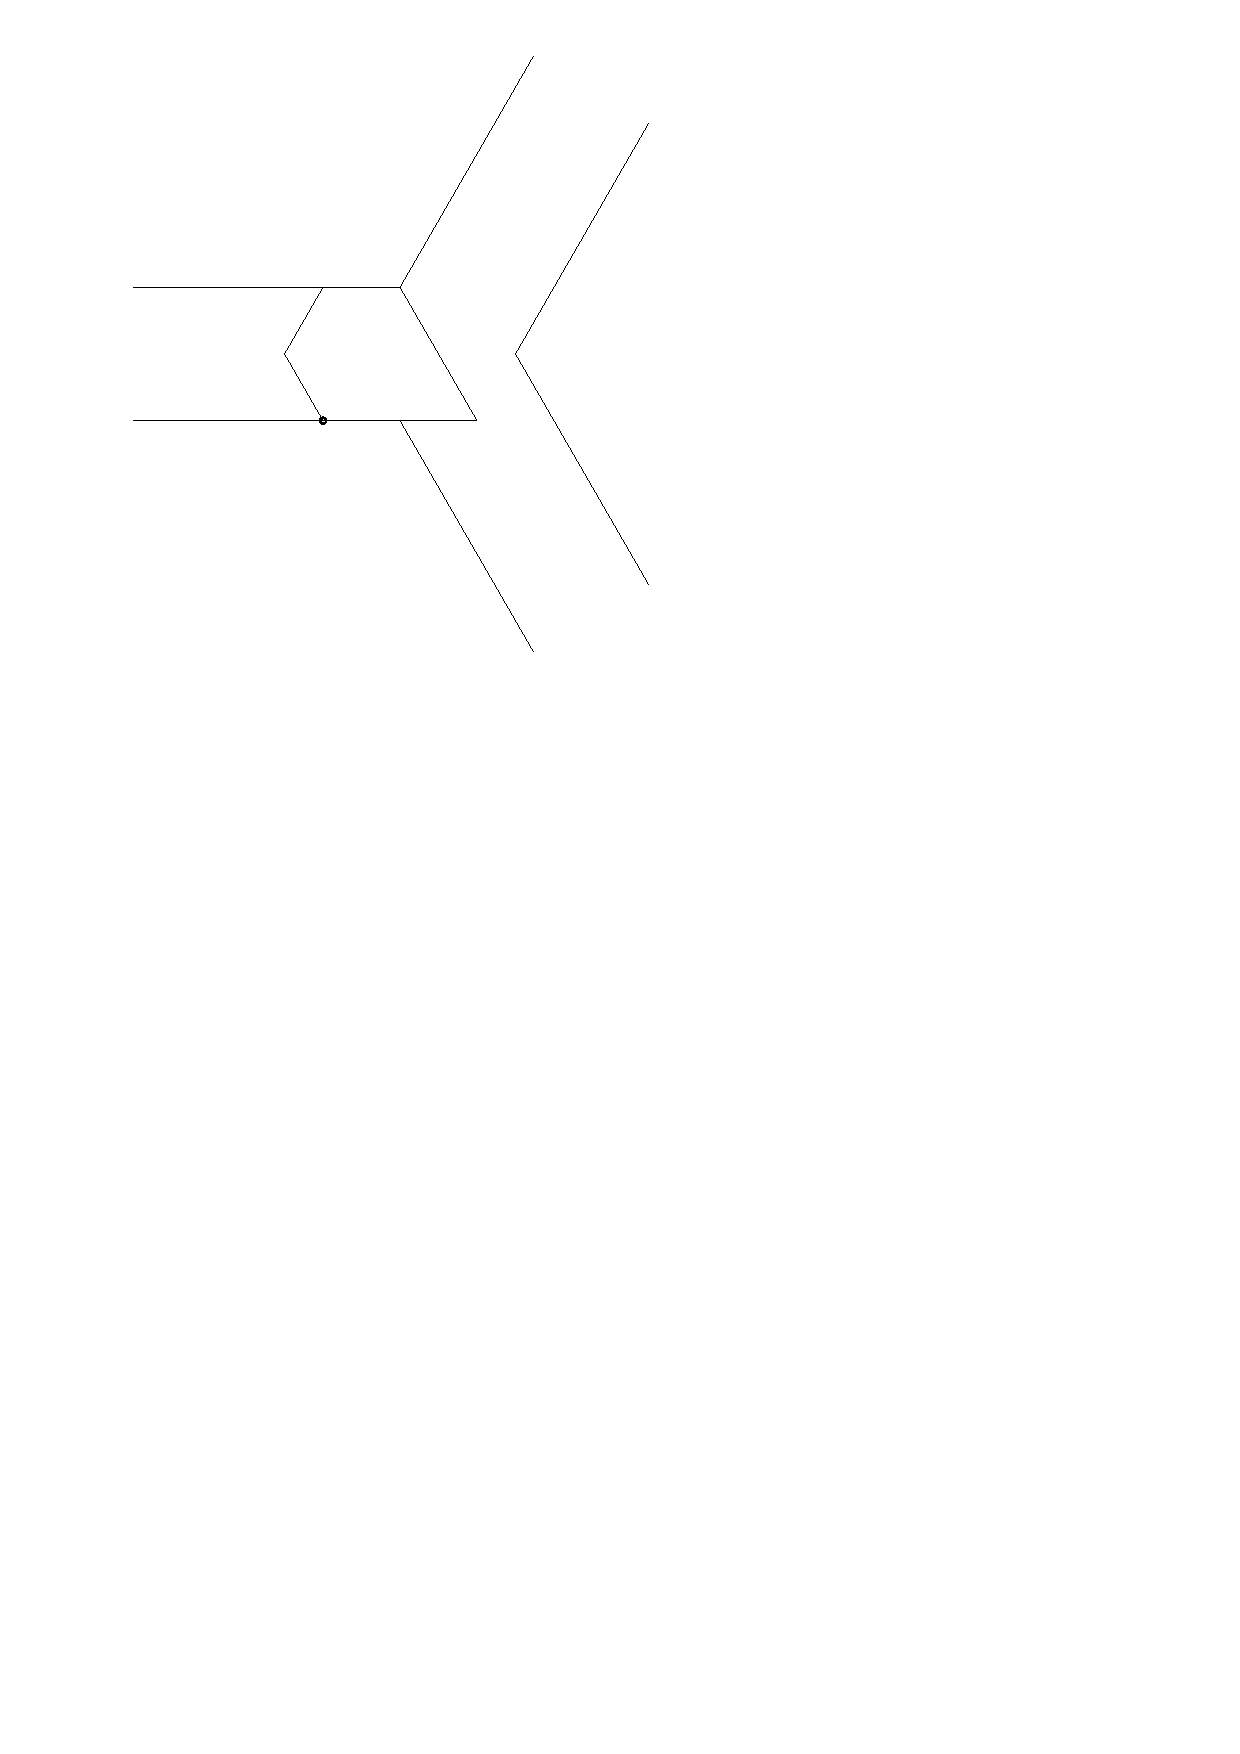
\includegraphics[width=\textwidth]{graphics/switchTerminalFinalized2.pdf}
% 	  \caption{A pentagon that is pinned in a channel junction that is formed by the sides of 3 
% large regular hexagons. It has two possible configurations, much like that of \ref{fig:linkage-1}}
% 	  \label{fig:linkage-2-1}
%   \end{subfigure}
%   \begin{subfigure}[b]{0.49\textwidth}
% 	  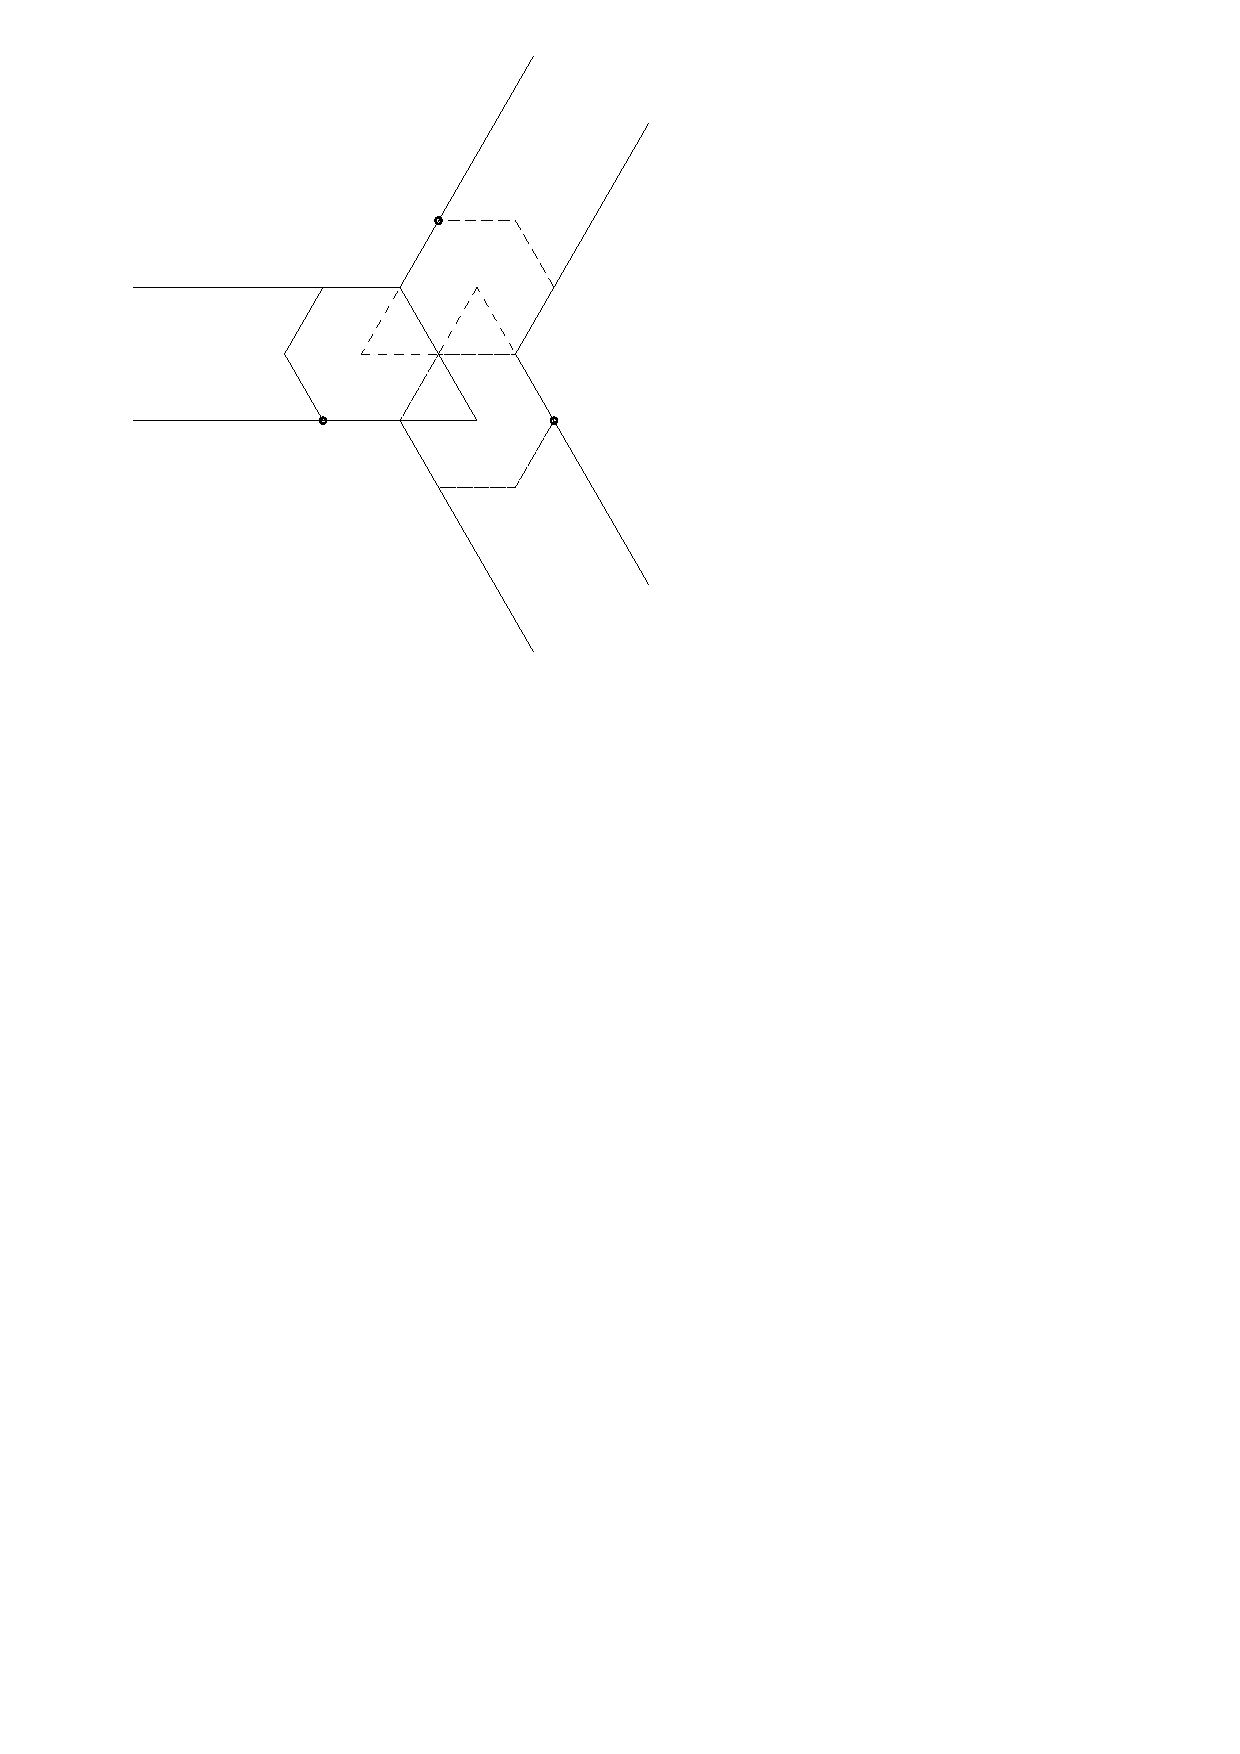
\includegraphics[width=\textwidth]{graphics/switchTerminalFinalized3.pdf}
% 	  \caption{A pinned pentagon residing in a channel junction that is formed by the sides of 
% 3 large regular hexagons with 2 dashed pentagons intersecting it.}
% 	  \label{fig:linkage-2-2}
%   \end{subfigure}
% \caption{Suppose the channel formed is a junction of three regular hexagons.  The polygon partially 
% residing in the junction is a regular hexagon with an equalateral triangle appended at an edge.  
% This polygon would prevent other polygons (i.e. the dashed polygons) of the same shape residing in 
% the center of the channel without intersection. This demonstrates that a the configuration space 
% within a multichannel environment can have concurrency issues, i.e. some configurations cannot be 
% realizable.}
% \end{center} \label{fig:linkage-2}
% \end{figure}\newpage
% Expanding upon the idea of \ref{fig:linkage-1}, forming channels with junctions as shown in Figure 
% \ref{fig:linkage-2} can be formed as such by evenly spacing the edges of a hexagonal lattice.  
% Visually, it is shown that only one of three possible pentagons can reside in the channel at one 
% time.  By asserting certain conditions on the lattice, and extending the problem to a greater 
% region 
% of a hexagonal lattice, we will be able to pose a realizability problem of whether a configuration 
% $\mathcal{A}$ can be reconfigured to $\mathcal{B}$ by switching pentagons without violating 
% overlapped polygon conditions.
% %Radius of regular polygons 
% %\newdimen\R
% %\R=3cm
% % \begin{figure}[h] 
% % \begin{center}
% % \begin{tikzpicture}
% % \begin{scope}
% % \filldraw[pattern=hexagons]  (0:\R) \foreach \x in {60,120,...,359} {
% %                 -- (\x:\R)
% %             }-- cycle (90:\R);
% % \end{scope}
% % \end{tikzpicture}
% % \caption{A hexagonal lattice contained in a hexagon.}
% % \label{fig:lattice}
% % \end{center}
% % \end{figure}
% %\newpage
% 
% % \begin{definition}[Graph]\label{def:linkages-2}
% % An ordered pair $G = (V, E)$ comprising a set $V$ of vertices or nodes together with a set $E$ of 
% edges or lines
% % \end{definition} 
% % \begin{definition}[Linkage]\label{def:linkages-1}
% % A collection of fixed-length 1D segments joined at their endpoints to form a graph.
% % \end{definition} 
% % A linkage can be thought of as a type of path-connected graph, i.e. the segments of a linkage are 
% the edges of a graph, and the endpoints of the segments are the vertices. For this paper, we 
% restrict our self to linkages that are simple planar graphs, i.e. a linkage that:
% % \begin{itemize}
% % \item[\rn{1}] does not have multiple edges between any pair of vertices,
% % \item[\rn{2}] does not have edges that cross, or
% % \item[\rn{3}] have loops (i.e. $(v,v) \in E$).
% % \end{itemize}  
% % \begin{definition}[Cycle]\label{def:linkages-3}
% %  A closed walk with no repetitions of vertices or edges allowed, other than the repetition of the 
% starting and ending vertex
% % \end{definition} 
% % \begin{definition}[Configuration]\label{def:linkages-6}
% % A specification of the location of all the link endpoints, link orientations and
% % joint angles.\cite{demaine2008geometric}
% % \end{definition}
% % \begin{definition}[Configuration Space]\label{def:linkages-7}
% % The space of all configurations of a linkage.
% % \end{definition} 
% % A configurations space is said to be continuous if for any two configurations, $\mathcal{A}$ and 
% $\mathcal{B}$ of a linkage $L$, $\mathcal{A}$ can be continuously reconfigured to $\mathcal{B}$ such 
% that, the reconfigurations reside in the configuration domain, $L$ remains rigid throughout 
% reconfiguration (i.e. all links' lengths are preserved), and no violations of linkage intersection 
% conditions. 
% % \begin{definition}[Pinned Joint]\label{def:linkages-8}
% % A vertex of a graph (or linkage) that is fixed to a position in a plane.
% % \end{definition} 
% % \begin{definition}[Free Joint]\label{def:linkages-8}
% % A vertex of a graph (or linkage) that is not fixed to a position in a plane.
% % \end{definition} x
% % \begin{figure}[h]
% % \begin{center}
% % 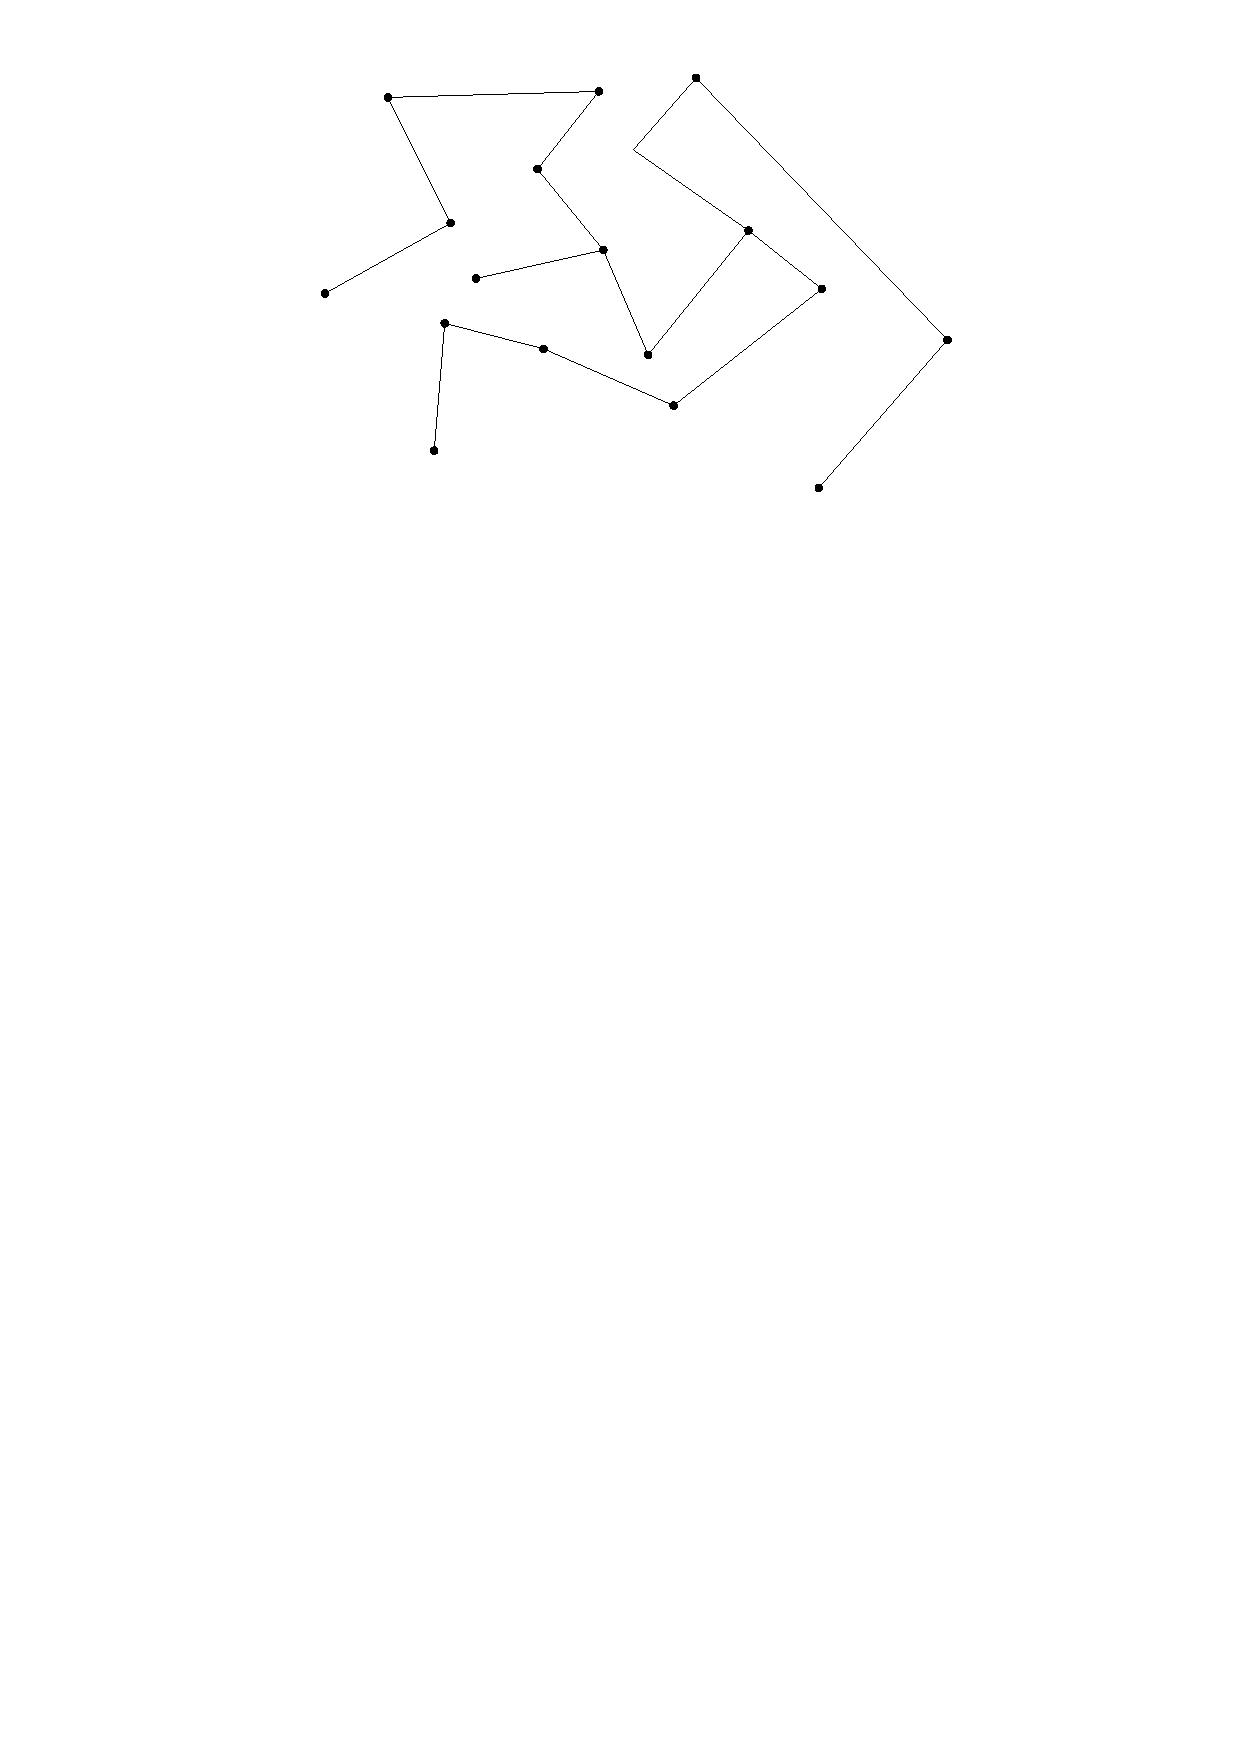
\includegraphics[scale=.5]{graphics/randomLinkage.pdf}
% % \end{center} 
% % \caption{A linkage with joints.}
% % \end{figure} 
% % \begin{figure}[h]
% % \begin{center}
% % 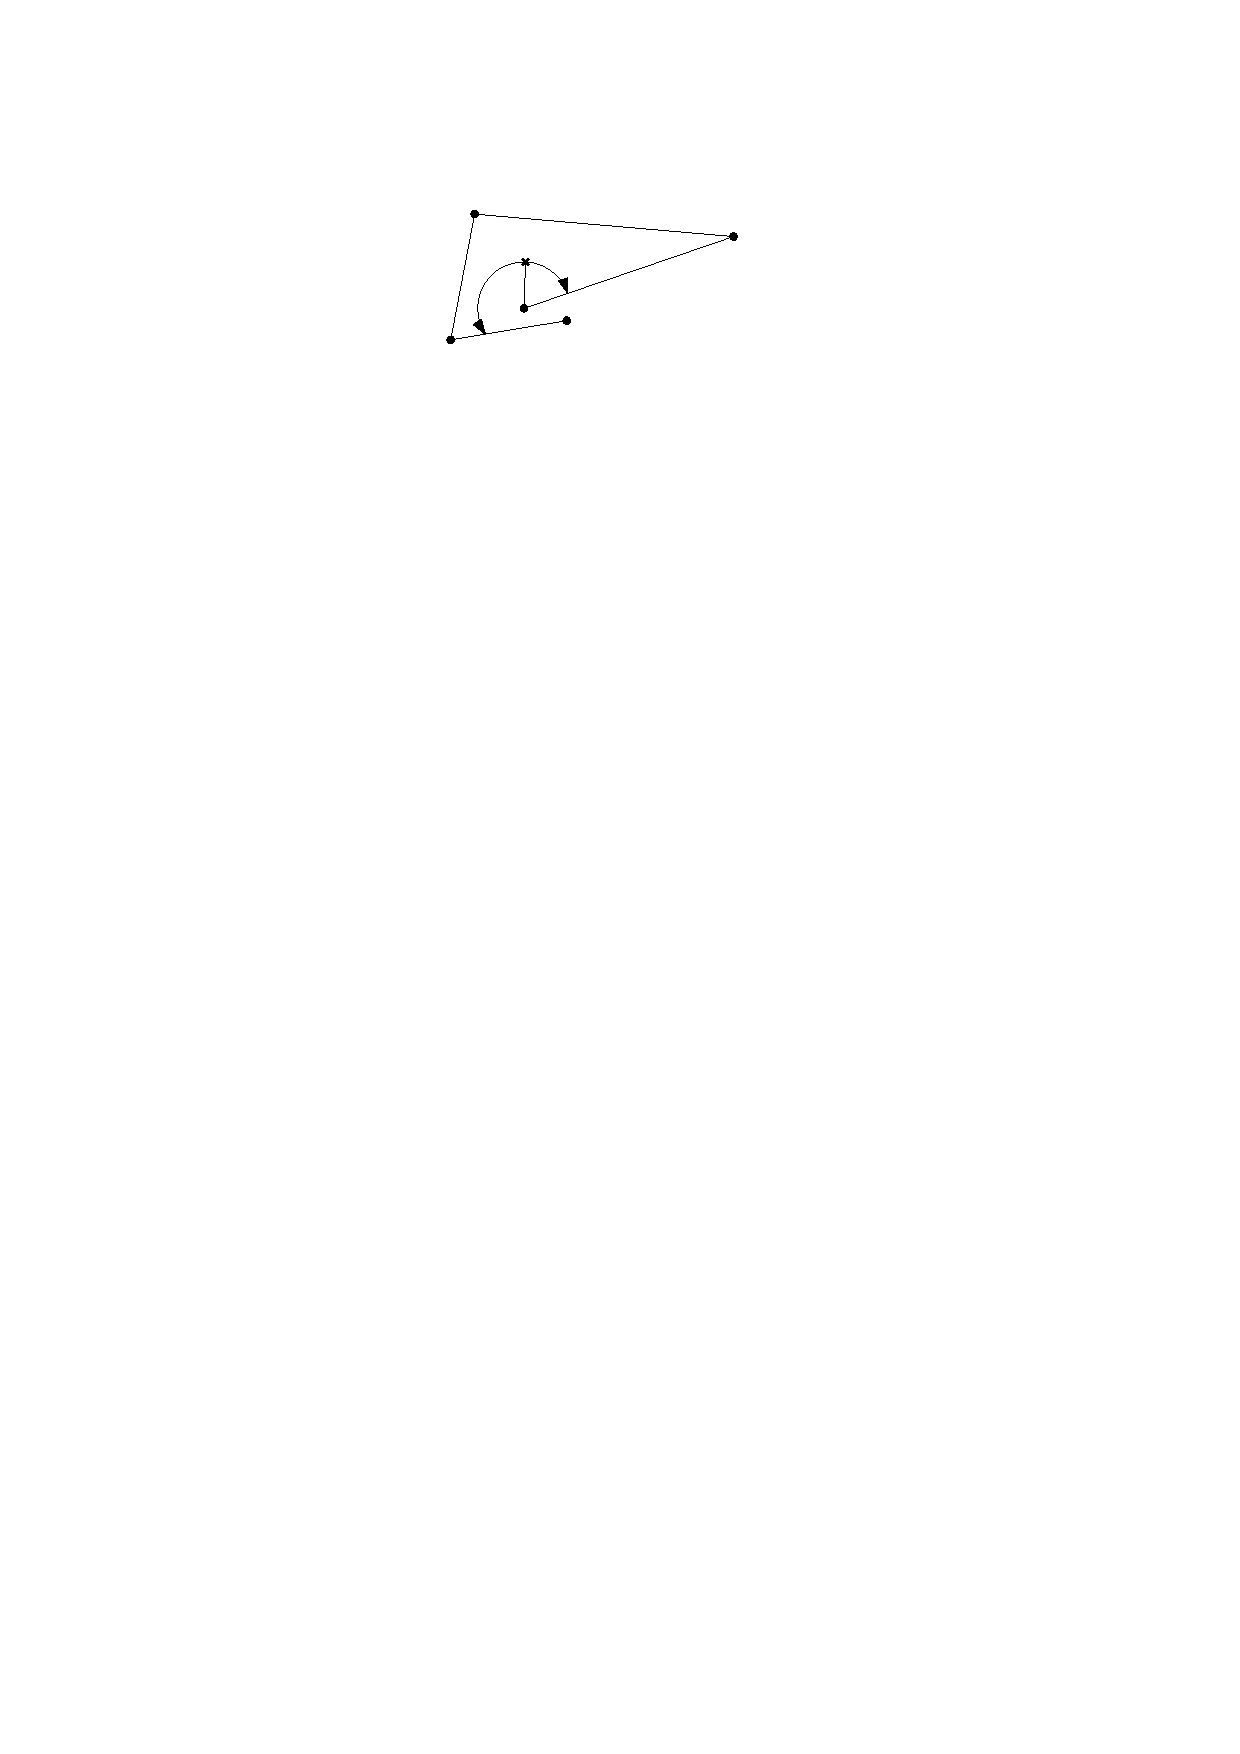
\includegraphics{graphics/freeJointPinnedJoint.pdf}
% % \end{center} 
% % \caption{The cross represents a free joint; the pinned joints are denoted as disks.  The range of 
% motion shown by the arc describes the continous configuration space of the linkage.}
% % \end{figure} 
% % 
% % For illustrations in the remainder of this paper, free joints will be represented as crosses and 
% pinned joints will be represented as disks.
